\documentclass[10pt,letterpaper]{article}

\usepackage{cogsci}
\usepackage{pslatex}
\usepackage{pdfsync}
\usepackage{apacite2}
\usepackage{amsmath}
\usepackage{graphicx}
\usepackage{topcapt}
\usepackage{color}
\usepackage{ upgreek }
%\usepackage{setspace}
%\singlespacing


\title{A Pragmatic Account of the Processing of Negative Sentences}
\author{{\large \bf Ann E. Nordmeyer} \\ \texttt{anordmey@stanford.edu}\\ Department of Psychology \\ Stanford University \\ 
\And {\large \bf Michael C. Frank} \\ \texttt{mcfrank@stanford.edu} \\ Department of Psychology \\ Stanford University \\ }

\begin{document}
\maketitle

\begin{abstract}

Previous work on sentence processing suggests that negative sentences are more difficult to process than positive sentences (e.g. \citeNP{hclark1972}), but that a supportive context can mitigate this effect (e.g. \citeNP{wason1965}).  We investigate the role of context on negative sentence processing by measuring the processing cost of negation with and without a visual context (Study 1) and then systematically varying the strength of the context (Study 2).  We find that context has a U-shaped effect on negation processing.  We then create a model to compute the informativeness of an utterance based on the context, and find that a model which considers both the surprisal of an utterance as well as the surprisal of a referent is highly correlated with participant reaction times.  This suggests that a theory of pragmatic surprisal can explain the processing cost of negation.  

\textbf{Keywords:} 
Negation; sentence processing; pragmatics
\end{abstract}

%%%%%%%%% INTRO %%%%%%%%% 
\section{Introduction}

%REVAMP TO FOCUS ON INFORMATIVENESS/PRAGMATICS HYPOTHESIS

Language is a powerful tool that allows us to describe not only the state of the world as we see it, but also the world as it is not.  If I am a regular at a coffee shop and always order chai, but the shop has run out today, the barista might say ``We don't have any chai today'' when I enter the shop.  Negative sentences are very informative when expectations are violated.

Although negation is critical for communicating many meanings, processing negation can be slow and effortful \cite{hclark1972, carpenter1975, just1971, just1976}. In EEG experiments, sentences where the final noun is semantically unexpected elicit an N400 response, and this response is found even when a negative makes the sentence logically true---suggesting that negation is slow to integrate with the rest of the sentence (CITES).  Similar results have been found in probe-recognition tasks \cite{kaup2003, kaup2006, hasson2006}.  Collectively this work suggests that negative sentences can be quite difficult to process.
 
There is a critical difference, however, between evaluating a sentence in the lab and comprehending speech in the real world. According to Grice's Cooperative Principle \cite{grice1975}, speakers should be truthful, relevant, and informative when speaking.  Negative sentences presented without context violate this principle.  If a barista says ``we don't have chai today'' to a customer who always orders coffee, this utterance would be neither relevant nor informative.  In general, negations are produced when there is some expectation that the speaker wishes to reverse.  

Congruent with this Gricean idea, a number of studies have shown that the difficulty processing negative sentences is mitigated by the presence of a supportive context \cite{wason1965, glenberg1999, ludtke2006, nieuwland2008, dale2011}. Some contexts are more effective than others at reducing processing demands, however. For example, contexts that explicitly mention a negated characteristic \cite{ludtke2006} or that present the negation within a dialogue \cite{dale2011} elicit faster reaction times, perhaps because the negation is more informative. But although these findings are congruent with the idea that pragmatic expectations are the source of negation's processing cost, they do not directly test that hypothesis.  The goal of our current work is to make such a test.

We propose that negative sentences are more informative in contexts that set up a strong expectation that is violated. If the processing cost of negation is pragmatic, then more informative negative sentences should elicit smaller reaction times. How should we quantify informativeness in context? Recent modeling work attempts to quantify pragmatic reasoning in simple experimental contexts \cite{frank2012,goodman2013}. The assumption underlying this work is that speakers are informative---they will produce utterances that will pick out smaller subsets of the context, leaving as little ambiguity as possible for the listener.  We use this definition of informativeness to provide a quantitative interpretation of our hypothesis.

To link informativeness---as computed in a probabilistic model---to reaction time, we assume that reaction time is proportional to \emph{surprisal}. Surprisal is an information-theoretic measure of the amount of information carried by an event (in this case, an utterance in some context). Surprisal has been used effectively to predict reaction times from probabilistic models \cite{levy2008}; this work provides inspiration for our current model. 

We test the hypothesis that pragmatic surprisal explains the processing cost of negative sentences. Study 1 measures this processing cost, replicating previous findings that context facilitates the processing of negation (Study 1).  Study 2 investigates the effect of the strength of the context by parametrically varying the base rate of a negated feature.  We compute the surprisal of sentences in these contexts, and find that a model of pragmatic informativeness predicts the relationship between context and reaction time.  These results support the idea that context affects negative sentence processing by modulating listeners' expectations. % trying to link back to the idea of expectations

\section{Study 1: Context vs. No Context}

To test whether non-linguistic contextual expectations alleviate the processing cost of negative sentences, we constructed a simple sentence verification task based on \citeA{hclark1972}.  Previous studies of the relationship between context and negation have required participants to actively engage with the context, either by describing pictures \cite{wason1965} or reading sentences \cite{glenberg1999}.  Here, participants passively viewed a visual context, eliminating linguistic confounds in previous work.  
 % This study explores whether a passively-viewed visual context is sufficient for facilitating the processing of negative sentences.  

\subsection{Method}

\subsubsection{Participants}

We recruited 100 participants to participate in an online experiment through the Amazon's Mechanical Turk (mTurk) website.\footnote{We programmed studies using Javascript, allowing us to collect reaction times for participants' responses.  Previous work has demonstrated that mTurk is an effective tool for collecting reaction time data \cite{crump2013}.}  Participants ranged in age from 18-65; 63 were male and 37 female.  We restricted participation to individuals in the United States. We paid participants 30 cents to participate, which took approximately 5 minutes to complete.  

\subsubsection{Stimuli}

\begin{figure}[t]
\begin{center} 
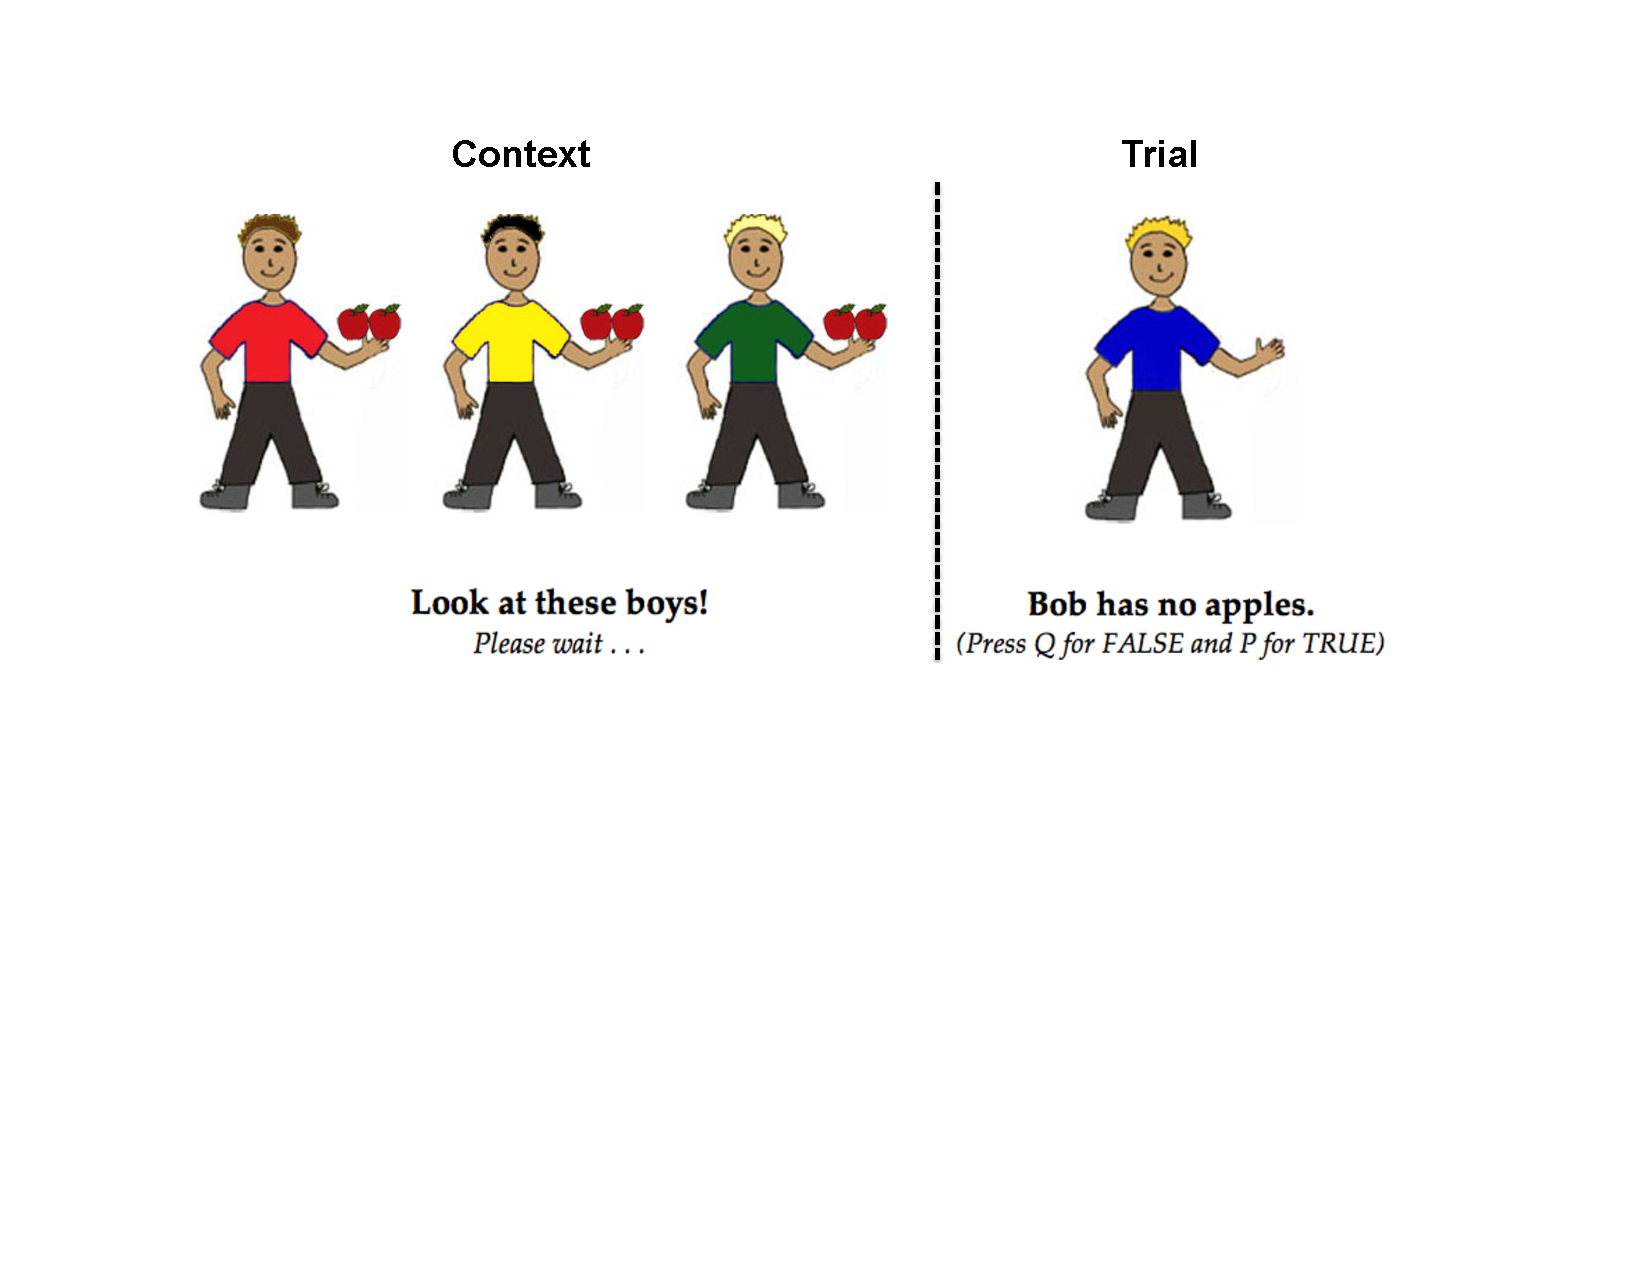
\includegraphics[width=3.25in]{figures/negatron_trialfig2.pdf}
\caption{\label{fig:trial} An example trial, consisting of two separate slides (shown sequentially): a context slide and a trial slide (true negative). }
\vspace{-5mm}
\end{center} 
\end{figure}

Twenty-eight trial items were created in which a character was shown holding either two of the same common, recognizable objects (e.g. two apples), or holding nothing.  On each trial, beneath the picture, was a sentence of the form ``[NAME] has/has no [ITEM].''  Half of the sentences were positive and half were negative, and they were paired with pictures such that half were true and half were false.  The experiment was fully crossed, with participants receiving 7 true positive, 7 false positive, 7 true negative and 7 false negative sentences over the course of the study.  Trials were presented to participants in a randomized order.  

Participants were randomly assigned to the ``no context'' condition or the ``context'' condition.  Participants in the no context condition saw a blank screen with a fixation cross in the center before each trial, while participants in the context condition viewed a context slide before each trial.  The context slide showed three characters, each holding two identical items.  The characters in the context all differed from the trial character and from each other in hair and shirt color.  The context slide instructed participants to ``Look at these [boys/girls]!''  An example of a context slide and a trial slide can be seen in Fig. \ref{fig:trial}.  


\subsubsection{Procedure}
%Cut this down - cut down practice trial info?
Participants were first presented with an instructions screen which described the task and informed them that they would be participating in a psychology experiment and could stop at any time.  Once they accepted the task, they were given eight practice trials with feedback. 
 % During the practice trials, a pop-up window informed participants if they were incorrect.  

In each trial, participants saw a context (3s) and then a picture and a sentence. They were asked to read the sentence and respond with a judgment of whether it was true or false when applied to the picture.  Participants were instructed to answer as quickly and accurately as possible.  We recorded reaction times for each trial, measured as the time from when the pictures/sentence were presented to the moment when the response was made.

%At the end of the experiment, participants were taken to a screen that collected demographic information.  Participants were required to enter their gender, age, and native language, and then were invited to provide optional comments about the task.  

\subsubsection{Data Processing}
%Put data processign stuff here - or maybe in Participants section???  Cut this down.

%%%REDO ANALYSES - TRIM OUTLIERS AFTER TAKING LOG RT
We excluded from analysis six participants who listed a language other than English as their native language, seven participants for having participated in a previous iteration of the experiment, and four participants for having an overall accuracy of below 80\%.  Thus, data from a total of 83 participants were analyzed.  We also excluded trials with RTs greater than 3 standard deviations from the log-transformed mean.  

\subsection{Results \& Discussion}

%I thought I would include a table of means for reproducibility, but it ends up looking pretty dense and cluttered.  I think I would rather include this in an appendix, or post on the lab website, for anyone interested in replication; otherwise most people reading the paper will find the graphs sufficient.  
%\begin{table}[t]
%\caption{\label{tab:e1means}Means and standard deviations of reaction times in milliseconds for each of the four trial types, for each of the two context conditions.}
%\begin{center}
%\small\addtolength{\tabcolsep}{-5pt}
%\begin{tabular}{ l  r  r  r  r } 
%\hline
%& \multicolumn{2}{c}{No Context} & \multicolumn{2}{c}{Context} \\
%  Trial Type & Mean& SD & Mean & SD \\ \hline                    
%True Positive & 1517 & 351 &  1509 & 535\\
% False Positive & 1727 & 406 &  1599 & 479\\
% True Negative& 1806 & 376 & 1581 & 483\\
%  False Negative & 1719 & 317 & 1655 & 614 \\
%\hline
%\end{tabular}
%\end{center}
%\end{table}

\begin{figure}
\begin{center} 
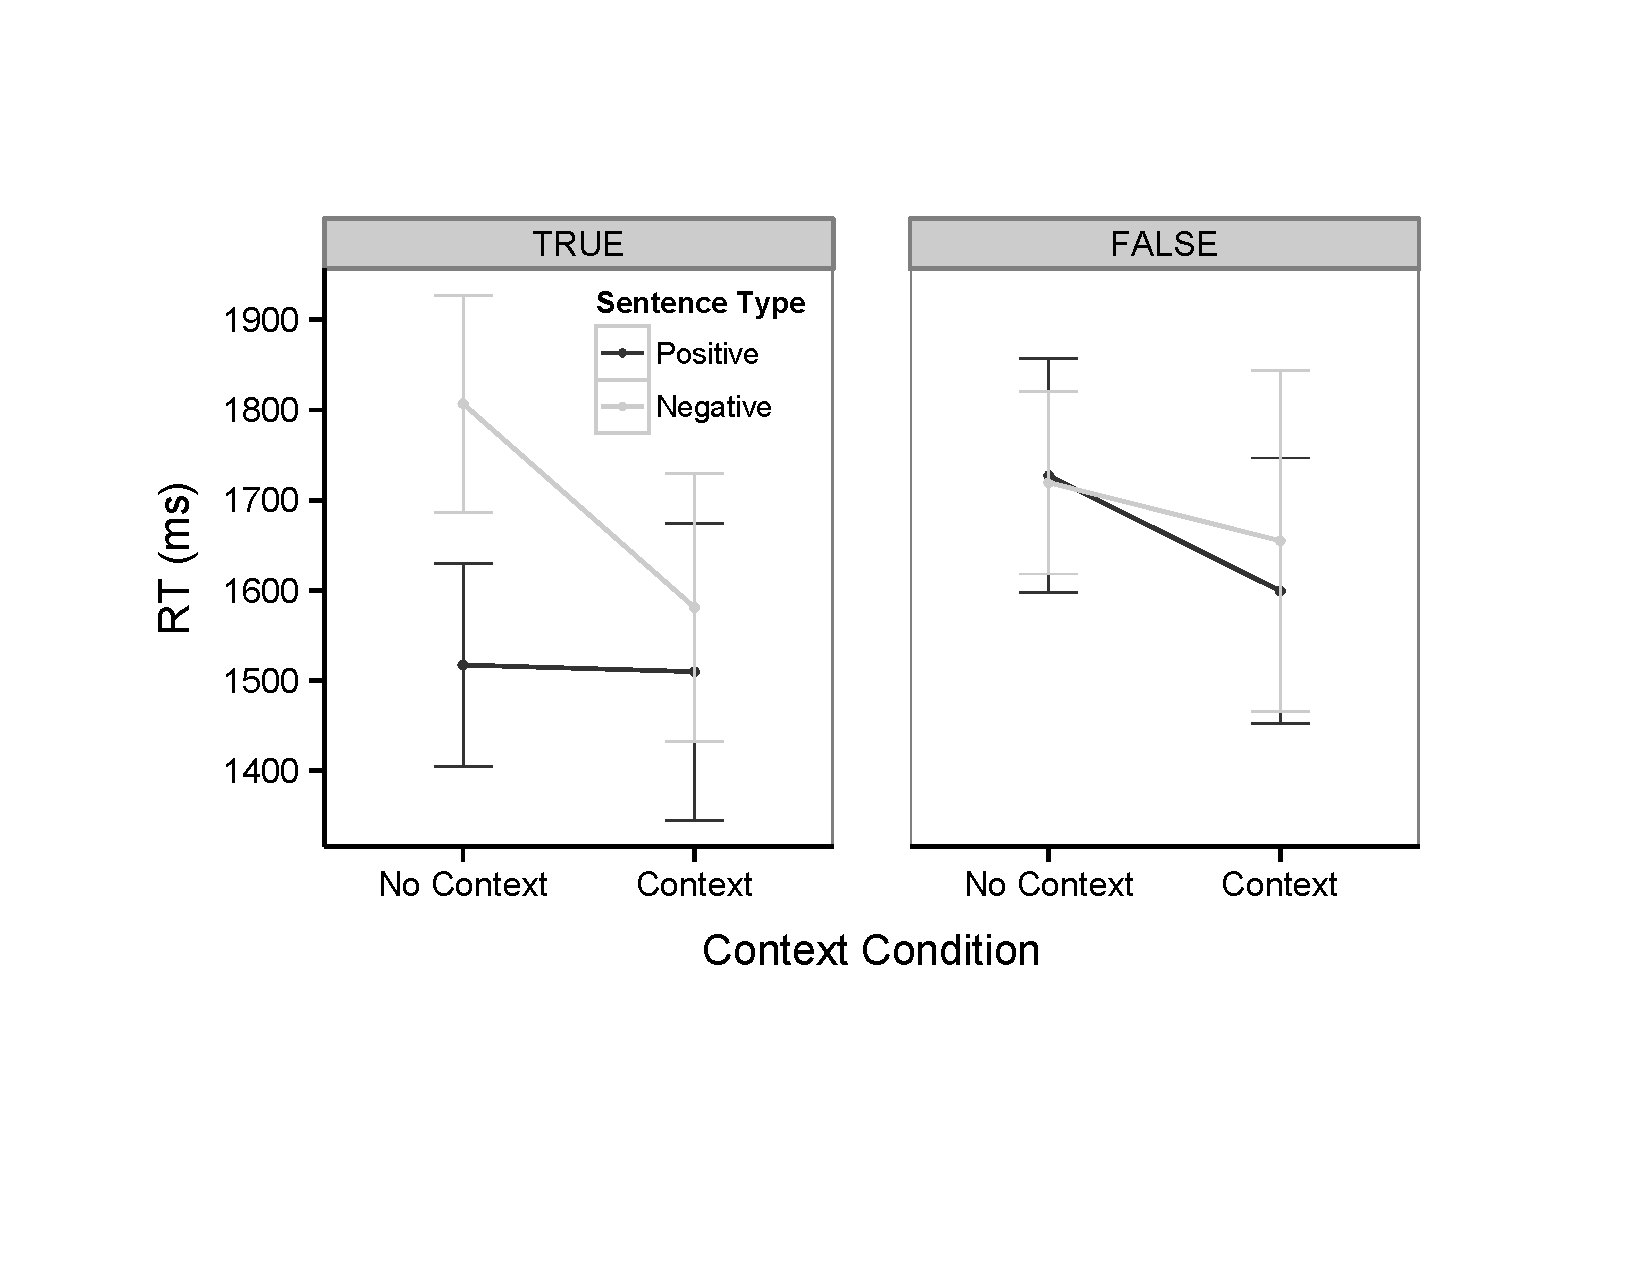
\includegraphics[width=3.25in]{figures/study1_linegraph.pdf}
\caption{\label{fig:e1line} Reaction times for each trial type, across different conditions.  Responses to true sentences are shown on the left, and false sentences are shown on the right.  Negative sentences are shown in grey, and positive sentences in black.  Error bars show 95\% confidence intervals.}
\end{center} 
\end{figure}

%\begin{table}[t]
%\caption{\label{tab:e1model} Coefficient estimates from a linear effects model estimating the effects of context condition, sentence type, and response on reaction time, accounting for random effects of participant and item.}
%\begin{center}
%\small\addtolength{\tabcolsep}{-5pt}
%\begin{tabular}{ r  r  r  r  } 
%\hline
% & Coefficient & Std. Err. &  $t$ value \\ \hline 
%  Intercept & 1727 & 75 & 22.91 \\ 	            
%Sentence Type(Negative) & -4 & 48 & -0.09\\
%Truth Value(True) &  -207 & 44 & -4.70\\
%Context Condition(Context) & -130 & 100 & -1.30\\
%Sentence Type $\times$ Context Condition & 53 & 68 & 0.78\\
%Sentence Type $\times$ Truth Value & 282 & 65 & 4.34\\
%Context Condition $\times$ Truth Value &  118 & 62 & 1.91\\
%Sentence $\times$ Context $\times$ Truth Value & -249 & 90 & -2.78\\
%\hline
%\end{tabular}
%\end{center} 
%\end{table}



%%%REDO RESULTS SECTION - PUT MAIN FINDINGS FIRST

<<<<<<< HEAD
Study 1 examined the effect of a visual context on the processing of negative sentences.  We found that true negative sentences were difficult to process when presented without context; in context, this effect disappeared (Fig. \ref{fig:e1line}).  This result is congruent with previous work on sentence verification, which has also found an interaction between negation and the truth value of a sentence \cite{hclark1972, carpenter1975, just1971, just1976}.  It is also congruent with work examining the effect of context on negative sentence processing \cite{wason1965, glenberg1999, ludtke2006, nieuwland2008, dale2011}.  

To examine the reliability of these findings, we fit a linear mixed-effects model to reaction times in response to sentences.  We examined the interaction between sentence type, truth value, and context on reaction times.\footnote{All mixed-effects models were fit using the lme4 package in R version 2.15.3.  The model specification was as follows: \texttt{RT $\sim$ sentence~$\times$~truth~$\times$~context + (sentence~$\times$~truth~\textbar~subject) +  (sentence~$\times$~truth~\textbar~item)}.  Significance was calculated using the standard normal approximation to the $t$ distribution \cite{barr2013}.}  Results of this model show a main effect of truth value, with significant faster reaction times for true sentences compared to false sentences ($\beta= -196$, $p< .001$).\footnote{Coefficient weights are interpretable in milliseconds.}  Although there was no main effect of negation across both conditions, there was an interaction between sentence type and truth value ($\beta= 260$, $p< .001$), replicating the finding that participants respond fastest to true positive sentences but slowest to true negative sentences  \cite{hclark1972}.  However, there was a significant 3-way interaction between context condition, sentence type, and truth value ($\beta= -227$, $p< .01$), suggesting that this interaction was primarily driven by the slow RTs for true negative sentences in the no context condition.  
=======
Negative sentences were difficult to process when presented without context; in context, this effect disappeared \ref{fig:e1line}.  This result is congruent with previous work on sentence verification, which has also found an interaction between negation and the truth value of a sentence \cite<e.g.>{hclark1972} and with work on the role of context in negation \cite<e.g.>{wason1965, nieuwland2008, dale2011}.  

To examine the reliability of these findings, we fit a linear mixed-effects model to participants' reaction times.  We examined the interaction between sentence type, truth value, and context on reaction times.\footnote{All mixed-effects models were fit using the lme4 package in R version 2.15.3.  The model specification was as follows: \texttt{RT $\sim$ sentence~$\times$~truth~$\times$~context + (sentence~$\times$~truth~\textbar~subject) +  (sentence~$\times$~truth~\textbar~item)}.  Significance was calculated using the standard normal approximation to the $t$ distribution \cite{barr2013}.}  Results of this model show a main effect of truth value, with significant faster reaction times for true sentences compared to false sentences ($\beta= -207$, $p< .001$).\footnote{Coefficient weights are interpretable in milliseconds.}  Although there was no main effect of negation across both conditions, there was an interaction between sentence type and truth value ($\beta= 282$, $p< .001$), replicating the finding that participants respond fastest to true positive sentences but slowest to true negative sentences.  Critically, there was a significant 3-way interaction between context condition, sentence type, and truth value ($\beta= -249$, $p< .01$), suggesting that this interaction was primarily driven by the slow RTs for true negative sentences in the no context condition.  
>>>>>>> 791e1c06ddb43e8423aa2bbad97e35b8048f4cc7

To understand why context had the greatest effect on true negative sentences, consider what a true negative trial looks like to a participant in the no context condition.  These are trials in which the participant has no expectation about what the character might be holding, because no context was provided to set up such an expectation.  The participant would then see a picture of a boy, not holding anything, with the sentence ``Bob has no apples.''  These types of trials likely cause participants to falter because there is no reason for ``apples'' to be mentioned at all.  However, when a participant first views a context such as the one in Fig. \ref{fig:trial}, they can form an expectation that boys typically have apples.  Now, when the trial shows a boy with no apples, a sentence such as ``Bob has no apples'' makes sense.

Study 1 contributes to a body of evidence suggesting that negative sentences are more felicitous when they are used to negate an expectation, and that such expectations can be set up by an appropriate context.  In Study 2, we examine how systematically manipulating the context might produce changes in reaction times by altering the strength of the expectations created by the context.  

%\subsection{Discussion}

%Study 1 provides further evidence for the effect of context on the processing of negative sentences.  Several previous studies have shown that embedding negative sentences in a supportive linguistic context leads to faster processing of negative sentences \cite{wason1965, glenberg1999, ludtke2006, dale2011}.  In this study, we presented some participants with a visual context that was designed to set up an expectation for what the trial picture might look like.  We found that viewing these contexts before each trial lead to faster processing of negative sentences, with true negative sentences showing the greatest effect.  



\section{Study 2: Varying strength of context}

Should all contexts be equally helpful in processing negation? 
% In Study 2, we test the idea that negation processing is facilitated in contexts where negative sentences would be most informative.  In Study 1, the sentence ``Bob has no apples'' is highly informative in the context condition, because a boy with no apples violates the expectation that all boys have apples.  However, if only one of the boys in the context had apples, the sentence ``Bob has no apples'' is less informative because the expectation that boys will have apples is weaker.
In Study 2, we quantitatively manipulated the strength of the context.  Participants saw contexts consisting of either three (Study 2a) or four (Study 2b) characters in which some subset of the characters were holding the target item.  If the context gives participants a glimpse into the ``world'' that each trial exists in, this represents a small sample of the base rate of what the characters in this world look like.  By manipulating this base rate, we can change peoples' expectations about the trial character.  If the differences in reaction times between the no context and the context condition in Study 1 are due to the relative informativeness of the negative utterance based on the context, we should expect to see a relationship between the strength of the context and reaction time. 

\subsection{Method}

<<<<<<< HEAD
\subsubsection{Participants } 
We recruited 600 participants to participate in an online experiment through the mTurk website, 200 in 2a (129 male, 71 female) and  400 in 2b (205 male and 195 female). Participants ranged in age from 18-over 65.  We restricted participation to individuals in the United States. We paid participants 30 cents to participate in the study, which took approximately 5 minutes to complete.  
=======
\subsubsection{Participants} 

We recruited 600 participants from mTurk. Participants ranged in age from 18-over 65; in Study 2a 129 participants were male and 71 were female and in Study 2b 205 participants were male and 195 were female.  We restricted participation to individuals in the United States. As before, we paid 30 cents for this 5 minute study.  
>>>>>>> 791e1c06ddb43e8423aa2bbad97e35b8048f4cc7

\subsubsection{Stimuli}

\emph{Study 2a} used the same 28 trial items and sentence types as those used in Study .  A between-subjects context factor determined what type of context participants saw.  Context conditions showed $\frac{0}{3}$, $\frac{1}{3}$, $\frac{2}{3}$, or $\frac{3}{3}$ of the characters holding objects.  Trial stimuli were identical to those in Study 1.  

\emph{Study 2b} used 48 items.  The contexts were the same as in Study 2a, except that each context contained 4 boys and there were therefore 5 context conditions ($\frac{0}{4}$, $\frac{1}{4}$, $\frac{2}{4}$, $\frac{3}{4}$ or $\frac{4}{4}$).  

\subsubsection{Procedure}
 The procedure for Study 2a was identical to that of Study 1, with participants randomly assigned to condition.   In Study 2b, participants were given 4s (instead of 3s) to look at the context before the experiment automatically advanced.  This latency was changed to give participants more time to look at the slightly larger contexts; the procedure was otherwise identical.
 
 \subsubsection{Data Processing}
%Put data processign stuff here - or maybe in Participants section???  Cut this down.

%%%REDO ANALYSES - TRIM OUTLIERS AFTER TAKING LOG RT
<<<<<<< HEAD
We excluded from analysis 25 participants who listed a language other than English as their native language (9 in 2a and 16 in 2b), 24 participants for participating in a previous iteration of the experiment (3 in 2a and 21 in 2b), and 35 participants for having an overall accuracy of below 80\% (11 in 2a and 24 in 2b).  Thus, we analyzed data from a total of 177 participants in Study 2a and 339 participants in Study 2b. As in Study 1, we only analyzed correct trials and excluded trials with RTs greater than 3 standard deviations from the mean in log space.  
=======
We excluded 23 participants who listed a language other than English as their native language (7 in 2a and 16 in 2b), 36 participants for participating in a previous iteration of the experiment (15 in 2a and 21 in 2b), and 35 participants for having an overall accuracy below 80\% (11 in 2a and 24 in 2b).  Thus, we analyzed data from a total of 167 participants in Study 2a and 339 participants in Study 2b. As in Study 1, we only analyzed correct trials and excluded trials with RTs greater than 3 SDs from the log-transformed mean. 
>>>>>>> 791e1c06ddb43e8423aa2bbad97e35b8048f4cc7

Because we were interested in the effect of context, results from these two studies were combined and analyzed together, with context condition re-coded as a continuous variable by calculating the proportion of people in each context condition who had a target item (e.g. the $\frac{1}{3}$ condition in Study 2a was recoded as .33). 

\subsection{Results}
%NOTE: these means are not quite accurate and need to be updated if I decide to post them anywhere!
%\begin{table}[t]
%\caption{\label{tab:e2ameans} Means and standard deviations of reaction times in milliseconds for each of the four trial types, across each of the four contexts (none, one, two, three) for Study 2a (three-person contexts).}
%\begin{center}
%\small\addtolength{\tabcolsep}{-5pt}
%\begin{tabular}{ l  r  r  r  r  r  r  r  r} 
%\hline
%& \multicolumn{2}{c}{None} & \multicolumn{2}{c}{One}  & \multicolumn{2}{c}{Two}  & \multicolumn{2}{c}{Three}\\
%\hline
%  Trial Type & Mean & SD & Mean & SD & Mean & SD & Mean & SD \\ \hline                      
%True Positive & 1519 & 578 & 1412 & 612 & 1456 & 543 & 1487 & 592\\
% False Positive & 1685 & 668 & 1526 & 567 & 1489 & 475 & 1610 & 566\\
% True Negative& 1697 & 593 & 1629 & 666 & 1505 & 498 & 1600 & 560\\
%  False Negative & 1692 & 604 & 1543 & 602 & 1528 & 525 & 1737 & 672\\
%\hline
%\end{tabular}
%\end{center}
%\end{table}
%
%\begin{table}[t]
%\caption{\label{tab:e2bmeans} Means and standard deviations of reaction times in milliseconds for each of the four trial types, across each of the five contexts (none, one, two, three, four) for Study 2b (four-person contexts).}
%\begin{center}
%\small\addtolength{\tabcolsep}{-5pt}
%\begin{tabular}{ l  r  r  r  r  r  r  r  r r r} 
%\hline
%& \multicolumn{2}{c}{None} & \multicolumn{2}{c}{One}  & \multicolumn{2}{c}{Two}  & \multicolumn{2}{c}{Three} & \multicolumn{2}{c}{Four}\\
%\hline
%Trial Type & Mean & SD & Mean & SD & Mean & SD & Mean & SD & Mean & SD \\ \hline 	                
%True Positive & 1519 & 578 & 1412 & 612 & 1456 & 543 & 1487 & 592 & 1487 & 592\\
% False Positive & 1685 & 668 & 1526 & 567 & 1489 & 475 & 1610 & 566 & 1487 & 592\\
% True Negative& 1697 & 593 & 1629 & 666 & 1505 & 498 & 1600 & 560 & 1487 & 592\\
%  False Negative & 1692 & 604 & 1543 & 602 & 1528 & 525 & 1737 & 672 & 1487 & 592\\
%\hline
%\end{tabular}
%\end{center}
%\end{table}

\begin{figure}
\begin{center} 
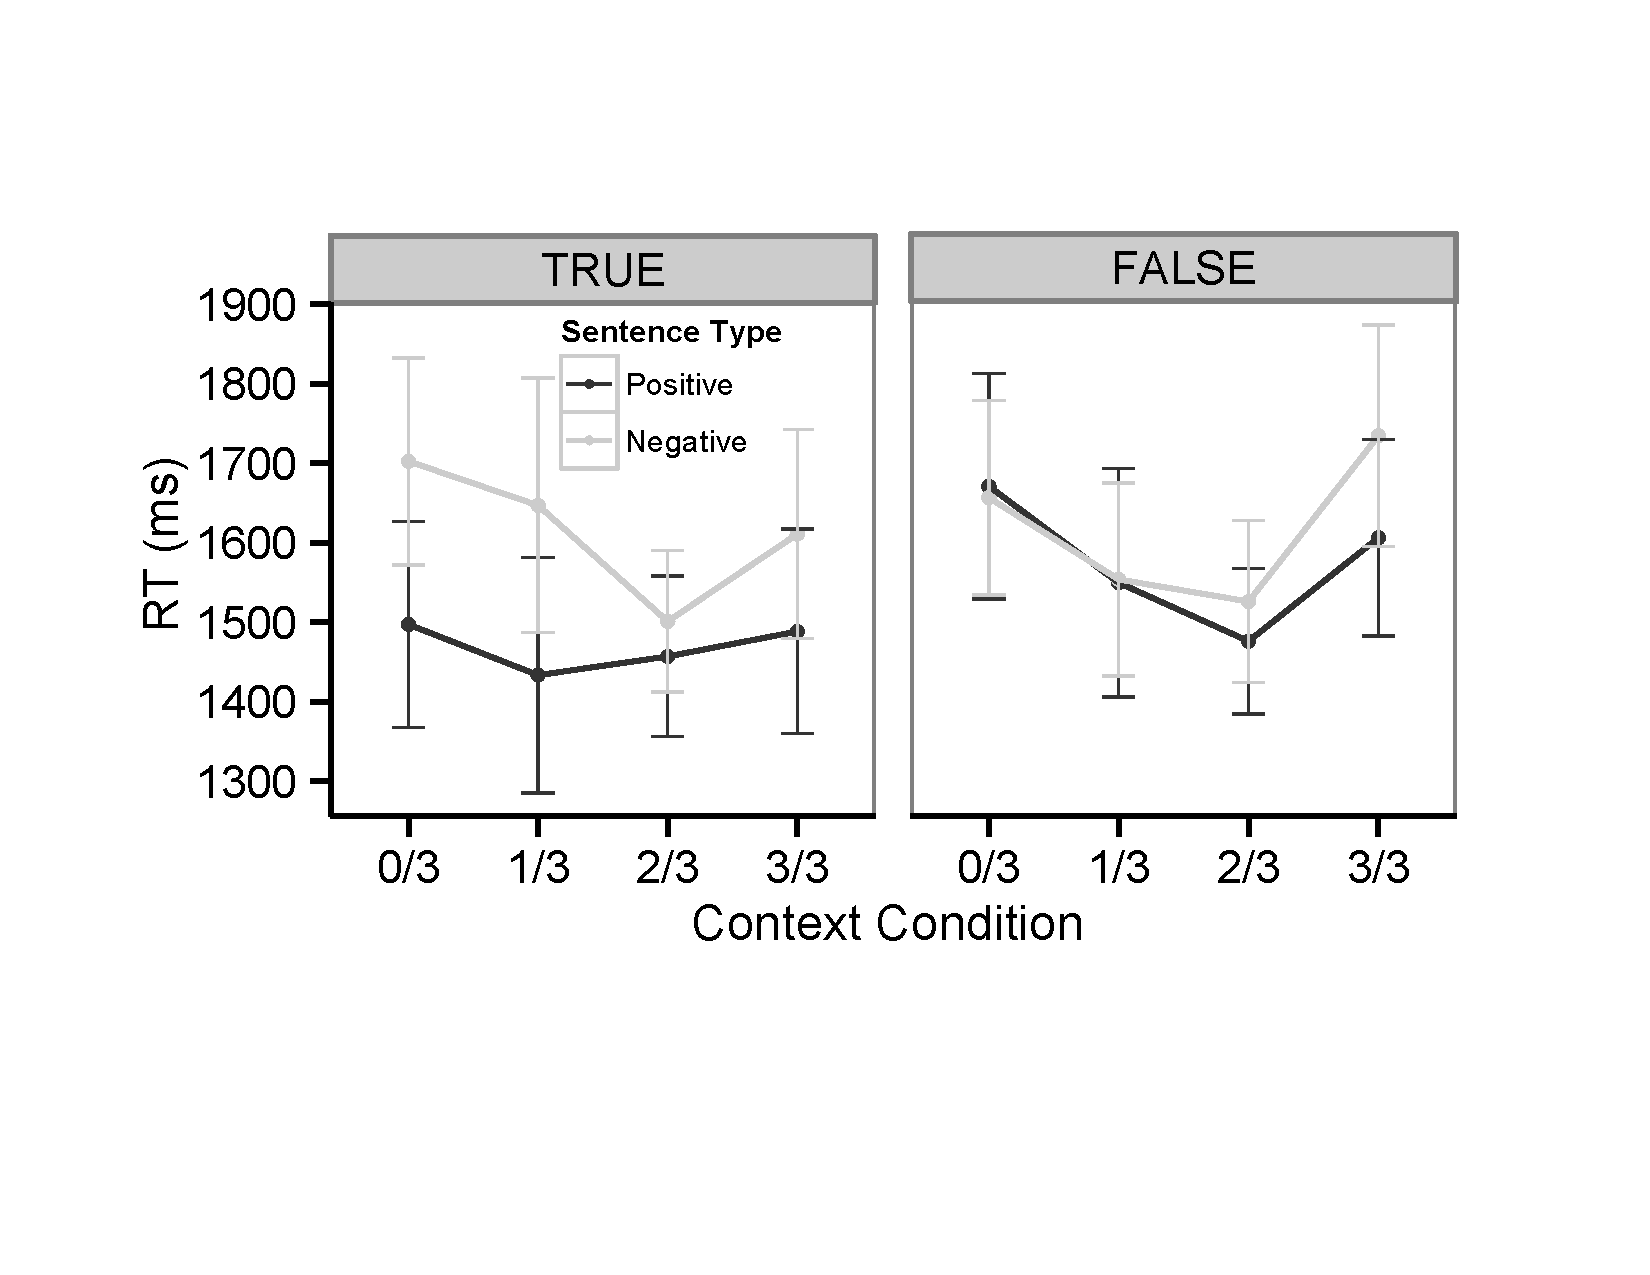
\includegraphics[width=3.25in]{figures/study2a_linegraph.pdf}
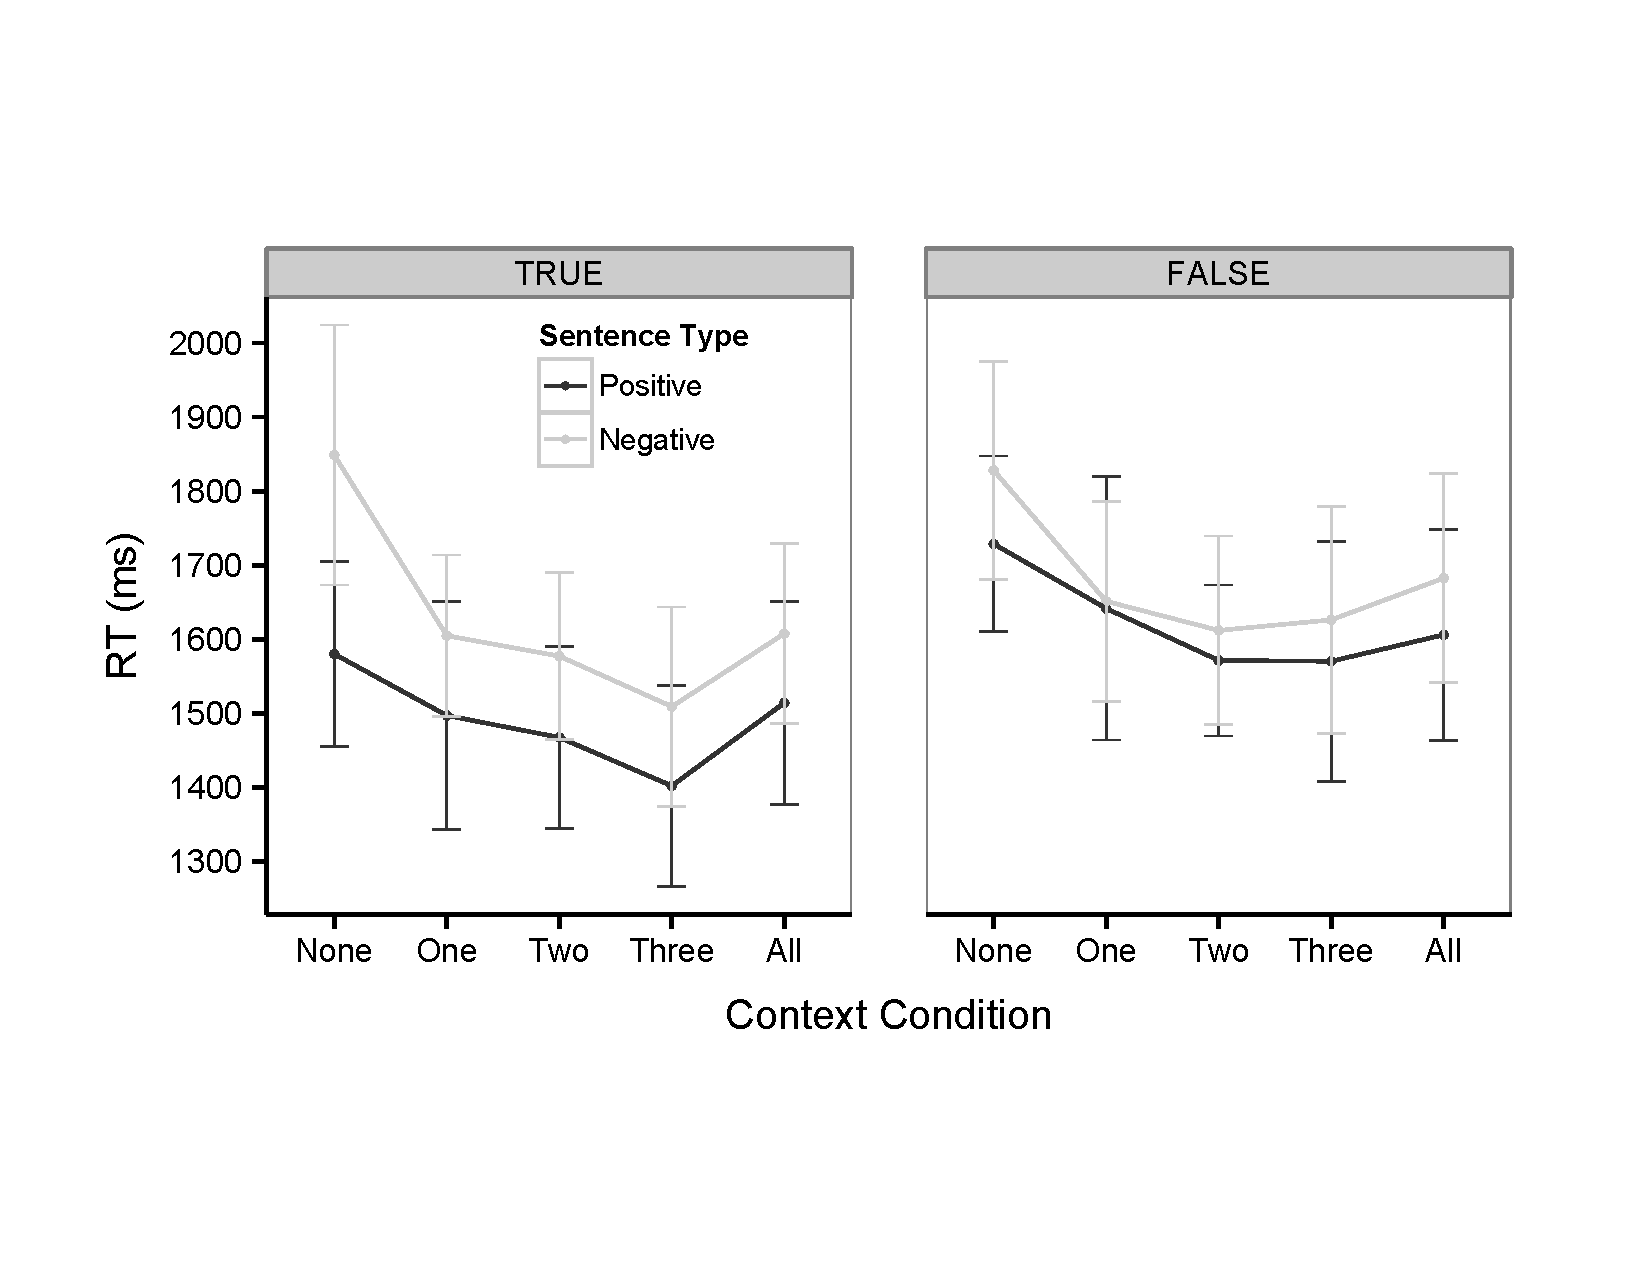
\includegraphics[width=3.25in]{figures/study2b_linegraph.pdf}
\caption{\label{fig:e2line} Reaction times for each trial type, across different conditions. Responses to true sentences are shown on the left, and false sentences are shown on the right.  Negative sentences are shown in grey, and positive sentences in black.  Data for Study 2a (3-person contexts) are shown above, and data for Study 2b (4-person contexts) are shown below.  Error bars show 95\% confidence intervals.  }
\end{center} 
\end{figure}

%\begin{figure}
%\begin{center} 
%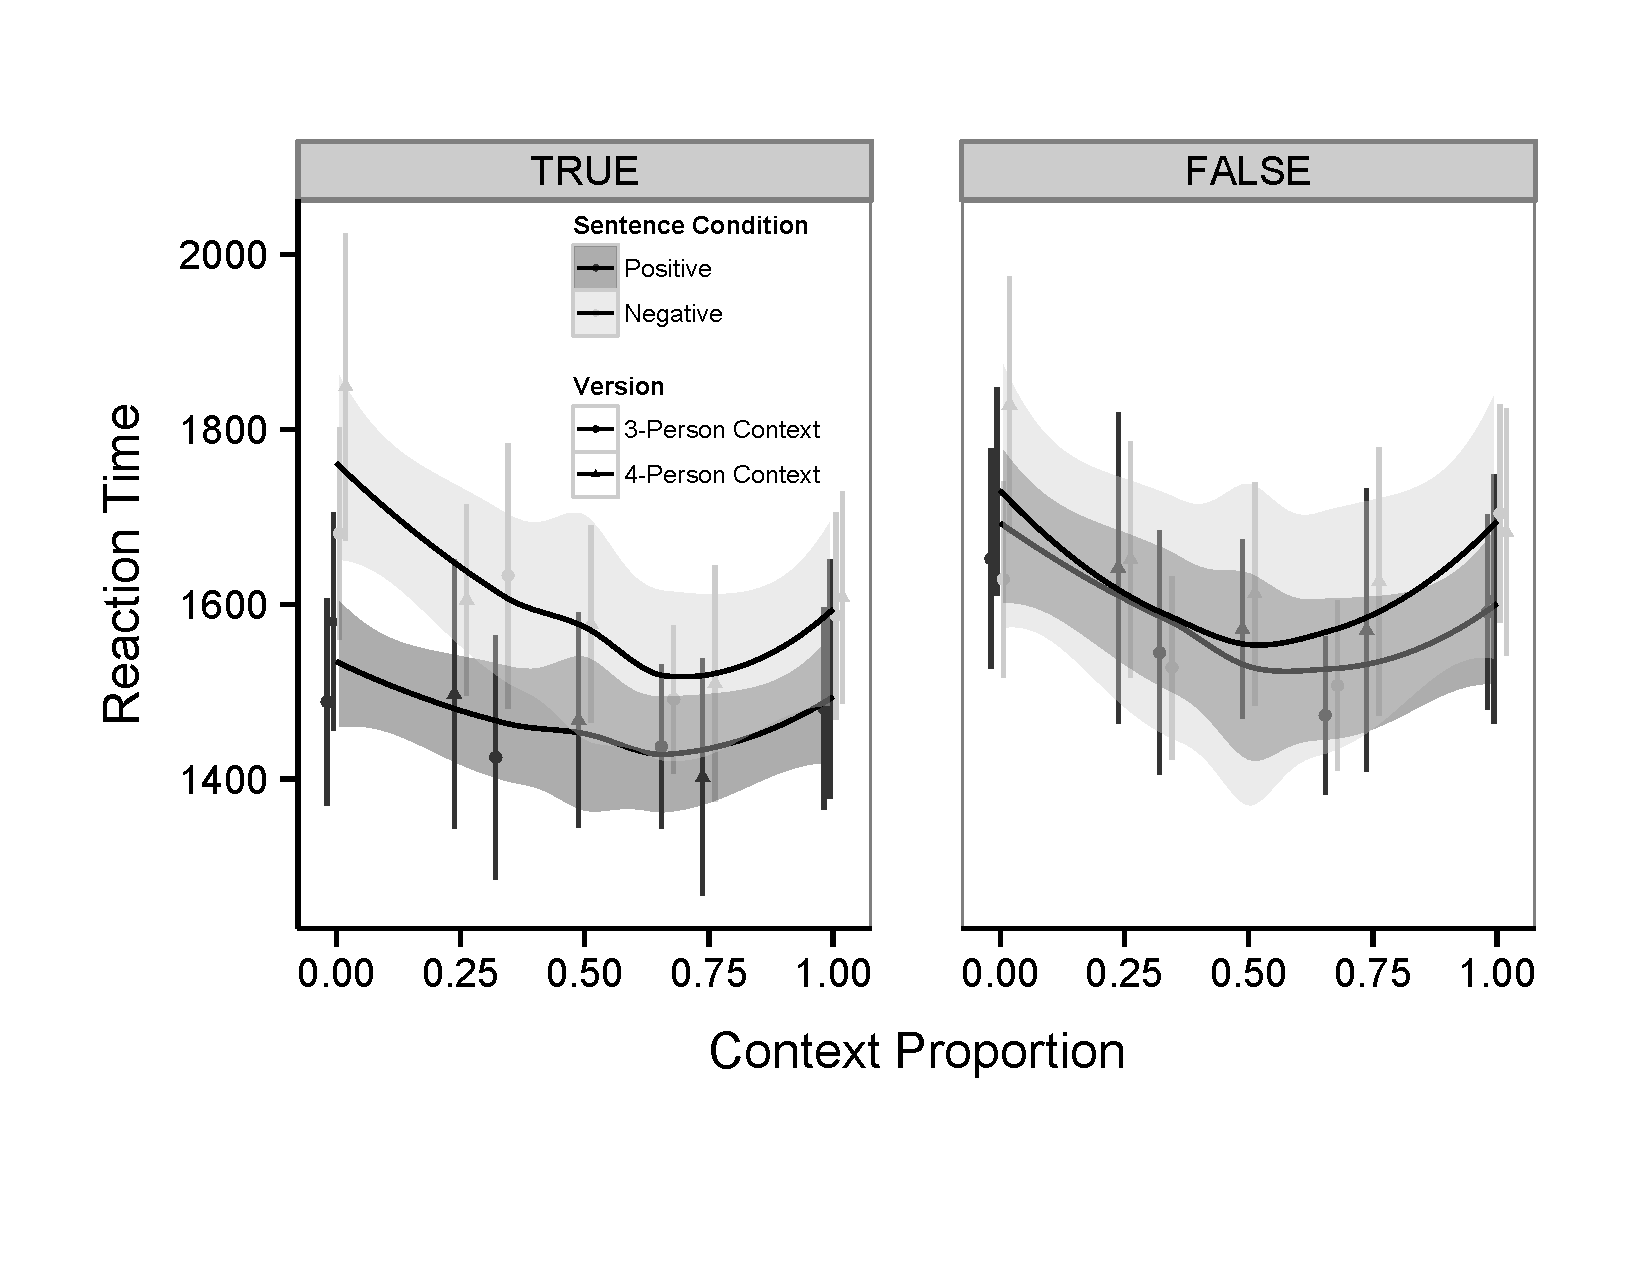
\includegraphics[width=3.25in]{figures/combined_plot.pdf}
%\caption{\label{fig:e2combined} Combined data for Studies 2a and 2b.  Reaction times for each trial type, across different context proportions (calculated as the proportion of people in the context with the target item).  Error bars represent the 95\% confidence intervals.}
%\end{center} 
%\end{figure}


%\begin{table}[t]
%\caption{\label{tab:e2model}Coefficient estimates from a linear effects model estimating the linear effects of context condition, sentence type, and response on reaction time for Studies 2a and 2b, accounting for random effects of participant and item.  The data from the two studies is combined, with context included as a continuous variable based on the proportion of characters in the context with the target item}
%\begin{center}
%\small\addtolength{\tabcolsep}{-5pt}
%\begin{tabular}{ r  r  r  r  } 
%\hline
%  \bf{Fixed Effects} & \bf{Coef.} & \bf{Std. Error} & \bf{t value} \\ \hline        
%  Intercept & 1702 & 34 & 49.91\\     
%Context(linear) &-167 & 33 & -5.02\\
%Sentence Type(Negative) &  42 & 28 & 1.5\\
%Truth Value (True) & -151 &   23 &  -6.54\\
%Context $\times$ Sentence Type& 29 &   37  &  0.78\\
%Context $\times$ Truth Value & 50  &   35  &  1.43\\
%Sentence Type $\times$ Truth Value &  162 &   35  &  4.67\\
%Context $\times$ Sentence $\times$ Truth Value & -160  &   50.35 &  -3.17\\
%\hline
%\end{tabular}
%\end{center}
%\end{table}

As the proportion of target items in the context increased, reaction times tended to decrease, particularly for negative and false sentences, supporting our hypothesis (Fig. \ref{fig:e2line}).  However, unexpectedly, reaction times increased slightly in the ``all'' condition, showing a U-shaped relationship between context and RT.  

We fit a linear mixed-effects model to reaction times in response to sentences.  We examined the interaction between sentence type, truth value, and context on reaction times.\footnote{The model specification was as follows: \texttt{RT $\sim$ sentence~$\times$~truth~$\times$~context + (sentence~$\times$~truth~\textbar~subject) +  (sentence~$\times$~truth~\textbar~item)}.}  As in Study 1, we found a significant effect of truth value, with significant faster reaction times for true sentences compared to false sentences ($\beta= -151$, $p< .001$).  Although there was not a significant main effect of negation, there was a significant interaction between sentence type and truth value, such that the difference between true positive and true negative was greater than the difference between the two types of false sentences ($\beta= 162$, $p< .001$).  There was also a linear effect of context, such that as the proportion of people with the target item in the context increased, reaction times decreased ($\beta= -167$, $p< .001$).  As before, there was a significant 3-way interaction between context, sentence type, and truth value, such that the linear effect of context was most striking in true negative sentences ($\beta= -160$, $p< .01$).

Responses in the $\frac{3}{3}$ and $\frac{4}{4}$ conditions suggest that the relationship between context and RT is not linear, however (Fig. \ref{fig:e2line}).  We added a quadratic term to our model to test for this nonlinear effect of context ($\beta= 696 $, $p< .001$).  The quadratic model fit our data significantly better in a likelihood comparison test ($\chi^{2}(1) = 71.25$, $p<.001$).  
% The contexts that had the most significant effect on processing time were those in which 60\%-75\% of the characters in the context had the target item; contexts in which all of the characters had the target item lead to slightly increased reaction times.    

Quantitative manipulation of the strength of the context resulted in systematic changes in the processing cost of negation, particularly for true negative sentences.  This finding is consistent with our initial hypothesis: As the proportion of people in the context with the target item increases, describing the trial picture as \emph{not} having that target item becomes more informative.  That is, the more people in the context who have apples, the more we expect a person with nothing to be described as ``a boy with no apples.'' 

%\subsection{Discussion}
%Study 2 was designed to further examine the effect of context on reaction time.  We hypothesized that as the strength of the context increased (i.e. the number of boys with apples in the context), reaction times would decrease.  We found a significant linear effect of context, consistent with our prediction.  We also found a significant quadratic effect of context.  Looking at the data, it appears that the contexts that had the most significant effect on processing time were those in which 60\%-75\% of the characters in the context had the target item; contexts in which all of the characters had the target item lead to slightly increased reaction times.    



%\section{Study 3: Measuring Listener Expectations}
%In studies 1 and 2, we demonstrated that a simple visual context can facilitate the processing of negative sentences, and that there is a linear (quadratic?) relationship between the strength of the context and the effect on reaction time to evaluate negative sentences.  Contexts that set up a strong expectation lead to faster reaction times to process a negative sentence when that expectation is violated.  Our prediction was based on previous work demonstrating that participants expect speakers to be informative when speaking \cite{frank2012}.  If everyone in the context has a specific feature, and the trial character is lacking that feature, it is highly informative to describe the trial character in terms of the negation of the expected feature.  However, although the results of Studies 1 and 2 support this interpretation, we do not know for sure whether participants expect speakers to use negation in these contexts.  Study 3 attempts to directly measure participants' expectations of how a speaker would describe the pictures seen in Studies 1 and 2, depending on the context.

%Our hypothesis here draws on the idea of \emph{surprisal}, a information-theoretic measure of the amount of information contained in an utterance.  Previous work has proposed that the processing difficulty of a word is the surprisal of that word, calculated as the -log of the probability of the word occurring in a given syntactic and semantic context \cite{levy2008}.  This theory proposes that expectations about what utterance a speaker will produce are related to a listener's speed to evaluate that sentence.  We draw on this theory in the realm of pragmatics, developing pragmatic theory of surprisal to explain the effect of context on the processing of negative sentences.  

%To test this theory, we conducted a study to evaluate participants' expectations of how a speaker would describe a picture in a given context.  Participants were introduced to an imaginary speaker who was described as either ``an honest guy who says things that are plausible and true'' or ``a tricky guy who says things that are plausible but false''.  This was originally set up to test participants expectations about false sentences; however, participants in the ``tricky'' condition struggled to understand this task, and results from this condition are not presented here.  Participants were then shown a set of three or four characters that the speaker ostensibly also saw (the contexts from the previous studies), and then shown a single character and asked to bet whether the speaker would use different sentences to describe the picture.  This allowed us to calculate the surprisal of positive and negative sentences based on participants' expectations about what sentences a speaker would use to describe these pictures, and determine if a relationship exists between the pragmatic surprisal of a sentence and reaction times to evaluate those sentences.  

%\subsection{Method}

%\subsubsection{Participants}
%280 participants were recruited to participate in an online experiment through Amazon's Mechanical Turk website.  Participants ranged in age from 18 - 65+, with the majority of participants being between 25 and 35 (109 participants).  167 participants were male and 113 were female.  Participation was restricted to individuals in the United States, and participants who indicated that their primary language was something other than English were excluded from analysis.  Participants were paid 30 cents to participate in the study, which took approximately 5 minutes to complete.  

%\subsubsection{Stimuli}
%A subset of 12 items out of the items used in Studies 1 and 2 were used for this study.  As in the previous studies, these items consisted of a context which presented either three (Study 3a) or four (Study 3b) characters who were either holding two of the same item or holding nothing, and a trial character who was presented alone holding either two items or holding nothing.  

%On each trial, participants were given four sentences to bet on.  The four sentences were always a positive sentence involving the target item, a negative sentence involving the target item, a positive sentence involving an alternative item, and a negative sentence involving an alternative item.  This meant that for pictures of a person holding a target item (e.g. a picture of a boy with apples), the two true sentence options were the positive-item sentence and the negative-alternative sentence (e.g. ``A boy with apples'' and ``A boy with no cookies'').  For pictures of a person holding nothing, the two true sentence options were the negative-item sentence and the negative-alternative sentence (e.g. ``A boy with no apples'' and ``A boy with cookies'').   

%\subsubsection{Procedure}
%As in Studies 1 and 2, participants were first presented with an instructions screen which described the task and informed them that they would be participating in a psychology experiment and could stop at any time.  Once participants accepted the task, they were introduced to the speaker, Joe, who was described as ``an honest guy who says things that are plausible and true''.  They were told that they would see different pictures, and their job was to decide how likely Joe is to use different sentences to describe the picture.  Participants were told that they could bet on more than one sentence, but that their bets must sum to 100.  

%Participants were then given two trials to practice betting.  Practice trials always showed a person with items, and did not include context slides.  Participants were reminded of the task on each trial.  During practice trials, participants were only given positive sentences to choose from, and only one of the sentences was true.  If participants bet on a false sentence, they were reminded that the speaker is an honest person who says things that are true.  This feedback was not given during test trials.

%Experiment trials differed from practice trials in that participants first viewed a context slide similar to the context slides presented in Studies 1 and 2.  Participants saw three (Study 3a) or four (Study 3b) characters with either none, one, two, three, or four of the characters holding target items with the rest of the characters holding nothing.  Beneath the characters, participants were told ``Joe sees these [boys/girls]''.  The context screen was displayed for four seconds and then the experiment automatically proceeded to the test trial for that item.  

%Test trials showed a single boy or girl either holding the same items or holding nothing.  Under the picture were four sentences (positive-item, negative-item, positive-alternative, and negative-alternative).  Participants were told to place bets on whether Joe would use these sentences to describe this picture, and were reminded that their bets must sum to 100.  

%\subsection{Results}
%\begin{figure}
%\begin{center} 
%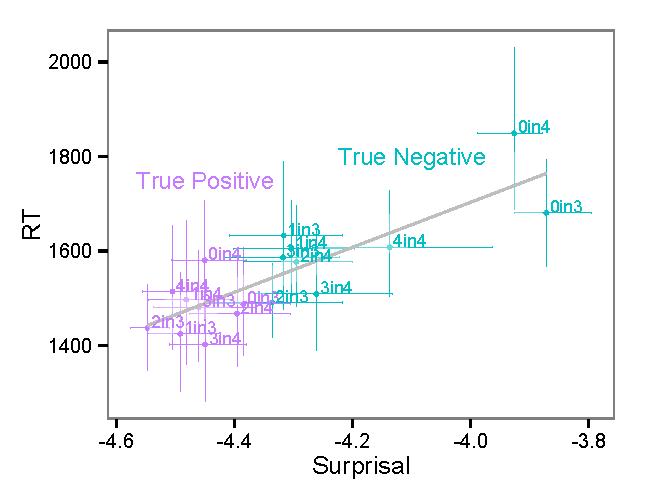
\includegraphics[width=3.25in]{figures/speakerstudy_comparison.pdf}
%\caption{\label{fig:e3plot} A comparison of surprisal from Study 3 (calculated as the -log of the mean bet on each sentence type) and reaction times from Study 2.  Error bars represent the 95\% confidence intervals.  }
%\end{center} 
%\end{figure}

%Study 3 was designed to test the effect of context on people's expectations of how a speaker would describe a picture.  We predicted that there would be a correlation between participants predictions of what a speaker would say to describe a picture, and reaction times to evaluate the predicted sentences.  

%Eleven participants who listed a language other than English as their native language were excluded from analysis.  Forty-six additional participants were excluded for having participated in a previous iteration of the experiment. Thus, data from a total of 223 participants were analyzed.  

%In each trial, participants had the ability to bet on four possible sentences: a positive sentence about the target item, a negative sentence about the target item, a positive sentence about an alternative item, and a negative sentence about the alternative item.  Any bets on sentences that were logically false were excluded; very few participants bet on false sentences (the average participant allocated less than 5\% of their bets to false sentences).  This eliminated all bets to alternative-positive sentences (e.g. ``A boy with cookies'' when the target item was apples), because these sentences were always false.  We also eliminated all bets to alternative-negative items (e.g. ``A boy with no cookies'' when the target item was apples).  Although these sentences were sometimes true (e.g. when the trial picture showed a boy with nothing), we were interested in seeing how participants bets on item negative sentences changed as the context changed.  Thus, we only analyzed bets to item-positive sentences when the trial picture showed a character holding the target items (e.g. bets on ``A boy with apples'' when the picture showed a boy holding apples) and bets to item-negative sentences when the trial picture showed a character holding nothing (e.g. bets on ``A boy with no apples'' when the picture showed a boy holding nothing).  These were analogous to the True Positive and True Negative sentences in Studies 1 and 2, allowing us to compare expectations about what a speaker would say to participants' reaction times in Study 2.  

%We used participants' expectations about how a speaker would describe a given picture to calculate surprisal, an information-theoretic measure that previous work has suggested is related to the processing difficulty of a word \cite{levy2008}.  Surprisal is calculated as the -log of the probability of a word given the context.  We calculated the probability of a word given the context by taking the mean bet for each sentence type (true negative and true positive, as described above) for each context condition, and took the -log of these mean bets to compute the surprisal of each sentence type for each context condition.  We then compared this measure of surprisal to the mean reaction times for true positive and true negative sentences for each context condition, as measured in Study 2.  A graph of this comparison can be seen in Figure \ref{fig:e3plot}.  There was a significant correlation between surprisal and reaction time in these data ($r=.82$, $p<.001$).  

%\subsection{Discussion}

%In Studies 1 and 2, we found that including a visual contexts facilitates the processing of negative sentences, and that this effect is modulated by the strength of the expectation set up by the context.  As the proportion of people with a target item in the context increases, the reaction time to process a negative sentence that negates that target property decreases.  We postulated that this effect is due to the ways that context changes expectations about what a speaker might say to describe a picture.  If you see a context in which the majority of boys are holding apples, and then see a boy holding nothing, it makes sense to predict that the boy holding nothing might be described as a ``boy with no apples''.  However, if you see a context in which nobody is holding anything, it would be odd to describe another person holding nothing as ``a boy with no apples'', because you have no reason to expect that he \emph{would} have apples.  Our prediction was that these expectations, calculated as the surprisal of seeing a picture described using a certain sentence, would be positively correlated with reaction times from previous studies.  Study 3 confirmed this hypothesis.  

%Why is it that different contexts influence our predictions of how a speaker might describe a picture?  Our initial hypothesis was built on work by Frank and Goodman (2012), who created a model of language comprehension based on the Grice's Maxim of Quantity, which dictates that speakers should choose utterances that are maximally informative.  This model demonstrated that listeners expect speakers to produce utterances that are highly informative.  With respect to this work, the utterance ``A boy with no apples'' is highly informative if it refers to a boy with nothing in a world where every other boy has apples, because this utterance uniquely identifies the intended referent.  However, in a world where none of the other boys are holding apples, the sentence ``A boy with no apples'' is uninformative, because it refers to every other boy in this hypothetical world.  In the next section, we test whether a model of informativeness can predict processing times for true positive and true negative sentences.  

\section{Model}

Studies 1 and 2 show that a simple visual context can facilitate the processing of negative sentences, with contexts that set up a strong expectation leading to faster reaction times for negative sentences.  Our hypothesis was that this effect is driven by the expectation that speakers are informative \cite{grice1975,frank2012}: If everyone in a context has a specific feature, and the target character is lacking that feature, it is highly informative to describe the trial character in terms of the negation of the expected feature. In this section, we formalize this prediction. Because of the Gricean nature of our prediction, we focus here on predicting the processing of true sentences.   

% Previous work has proposed that the processing difficulty of a word is the surprisal of that word, calculated as the -log of the probability of the word occurring in a given syntactic and semantic context \cite{levy2008}.  Here, we extend this theory to the realm of pragmatics. 

\begin{figure}[t]
\begin{center} 
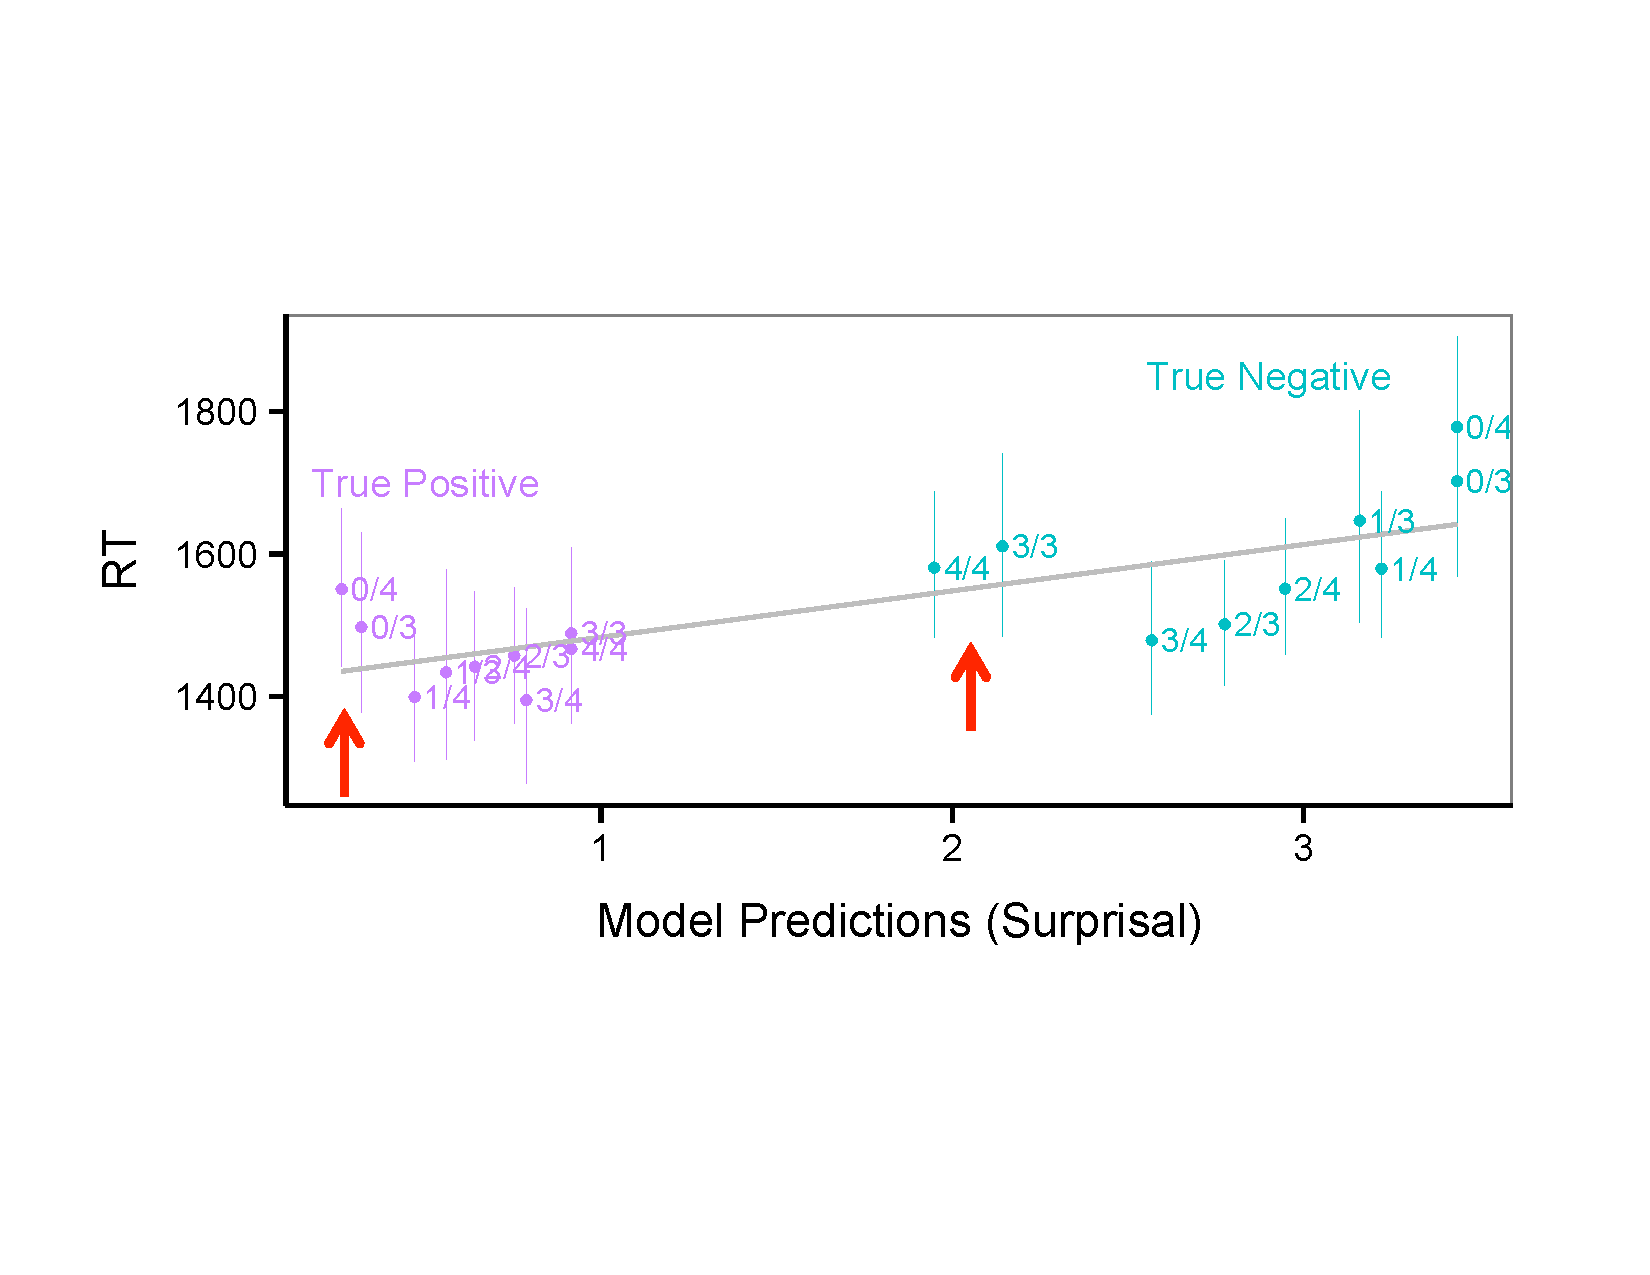
\includegraphics[width=3.25in]{figures/model1_comparison.pdf}
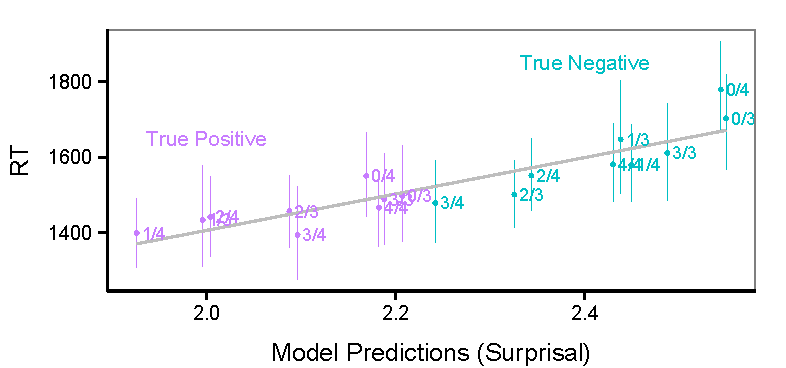
\includegraphics[width=3.25in]{figures/model2_comparison.pdf}
\caption{\label{fig:model1_sims} Best-fitting model predictions for a model of utterance surprisal (above) and a model of total surprisal, Equation \ref{eq:total} (below; fit to data from Study 2a and compared to full data set).  Positive sentences are represented in purple and negative sentences in blue.  Context conditions are identified as "xiny", where x is the number of characters with the target item and y is the total number of characters in the context (e.g. "1in3" for the 1/3 context).  Error bars show 95\% confidence intervals.}
\end{center} 
\end{figure}

We modeled the behavior of participants in our experiments (following \citeNP{levy2008}) by assuming that reaction time is proportional to the surprisal of the utterance $w$, given the context $C$ and the speaker's intended referent $r_S$:

\begin{equation}
RT \sim -\log(P(w| r_s, C)).
\end{equation}

\noindent We then define the probability of the message as proportional to its utility using a simple Luce choice rule (following \citeNP{frank2012}):

\begin{equation}\label{eq:pw1}
P(w | r_s, C) \propto  e^{\alpha U(w;r_s,C)},
\end{equation} 

\noindent where $\alpha=1$. This utility is defined as the informativeness of $w$ minus its cost:

\begin{equation}\label{eq:utility}
U(w;r_s,C) = I(w;r_s, C) - D(w).
\end{equation}

\noindent Informativeness in context is calculated as the number of bits of information conveyed by the word. We assume that $w$ has a uniform probability distribution over its extension in context (e.g. ``boy with apples'' applies to any boy who has apples, leading to a probability of $1/|w|$ of picking out each individual boy with apples) :

\begin{equation}\label{eq:info}
I(w;r_s, C) = -(-\log(|w|^{-1})).
\end{equation}

\noindent The cost term $D(w)$ can then be defined in any number of ways; in this model we define it as the number of words in the utterance multiplied by a cost-per-word parameter.  Note that in our experiment, the negative sentences always have exactly one word more than the positive sentences. 

Combining Equations \ref{eq:pw1}--\ref{eq:info}, and normalizing Equation \ref{eq:pw1} over all possible words in the vocabulary $V$, we have:

\begin{equation}\label{eq:pw2}
P(w | r_s, C) = \frac{ e^{\log(|w|^{-1}) - D(w)}} {\sum_{w' \in V}{e^{\log(|w'|^{-1}) - D(w')}}}.
\end{equation}

\noindent This model makes the prediction that as the number of e.g. boys with apples in the context increases, the informativeness of a negative sentences such as ``Bob has no apples'' increases, because the negative sentence selects an increasingly smaller subset of the context. Higher informativeness sentences will have higher probability, hence lower surprisal and faster RTs. 

% check cost param, compute significance
We fit this model to data from Study 2, with cost = 2 (CHECK, Figure \ref{fig:model1_sims}). The model accounted for a substantial amount of variance in participant reaction times ($r=.72$ **CALCULATE SIG.**).  The model accurately predicts that negative sentences have higher surprisal (slower reaction times), and captures many of the context effects.  Nevertheless, the model fails to capture the U-shaped relationship seen in Study 2; specifically, it underestimates the surprisal of $\frac{0}{3}$ and $\frac{0}{4}$ contexts for positive sentences, and $\frac{3}{3}$ and $\frac{4}{4}$ contexts for negative sentences.

In these trials, participants may have found the target picture surprising, regardless of the sentence that they read. For example, in $\frac{0}{3}$ and $\frac{0}{4}$ contexts followed by a true positive trial, this means that participants saw several boys with nothing, and then saw a boy holding something.  To account for reaction time related to seeing the target picture, we included the surprisal of the referent $r_S$ as well as the surprisal of the message $w$ given the referent. We estimated this probability via the count of the target property in the context, smoothed with a parameter $\lambda$:

\begin{equation}\label{eq:pp}
P(r_S | C) =  \frac{\# Matching People  + \lambda}{\# Total People + 2\lambda}
\end{equation}

We then added $-\log(p(r|C))$ (Equation \ref{eq:pp}) to $-\log(p(w|r_s,C))$ (Equation \ref{eq:pw2}), resulting in:

\begin{equation}\label{eq:total}
RT \sim - log(P(w|r_s, C)) - \beta ~ log(P(r_S|C)).
\end{equation}

\noindent Note that this formulation is quite similar to a model which accounts for the prior probability of the referent $p(r_S)$; the only difference is our use of a weight $\beta$ to adjust the different effects of these two probabilities.  

We fit this new model to the data from Study 2a only, which resulted in parameter values of $\text{cost} = .5$, $\lambda=.2$, and $\beta=.4$.  We then used these values to test model fit for the data from Study 2b.  The model provided a good fit to Study 2a and a similarly-strong parameter-free fit to Study 2b (see Table ****MAKE THIS TABLE****).  Fit to the full dataset is shown in Figure \ref{fig:model1_sims}.

\section{General Discussion}

What makes negation so hard? It takes longer to evaluate negative sentences than positive sentences when presented with no context, but these effects are mitigated in context. We suggested a Gricean account: the processing cost of negation is related to the degree to which it violates expectations about communication in context. In our studies, by changing the proportion of people in the context who held a target item, we systematically manipulated participants' contextual expectation.  We found a parametric relationship between the strength of the context and reaction times, and this relationship was well fit by a model of the surprisal of a sentence and its referent given the context.s.  

Previous work on sentence processing has suggested that processing negation is fundamentally difficult, perhaps due to the processing cost of negating a proposition (e.g. \citeNP{clark1972}) or the cost of suppressing an affirmative representation (e.g. \citeNP{kaup2003}).  Our work here suggests that the difficulty of negation may not be unique to negation at all; instead, general pragmatic mechanisms could be driving this effect.  Due to the specific pragmatics of negation, negative sentences presented without context are uninformative and are thus unlikely to be produced, leading to increased surprisal and slower processing times.  In conversation, however, negative sentences are often produced when some expectation has been violated, decreasing surprisal and processing time.  

Although our specific focus was to understand the processing of negative sentences, this work can be extended to quantify the effect that context has on sentence processing more generally.  Debates about the effects of pragmatics on linguistic processing exist in other domains as well (e.g. the processing of scalar implicatures, \citeNP{huang2009, huang2011, grodner2010}).  Formal models of pragmatics can shed light more generally on the role that context plays in linguistic processing. 

\section{Acknowledgments}
This material is based upon work supported by the National Science Foundation Graduate Research Fellowship. Any opinion, findings, and conclusions or recommendations expressed in this material are those of the authors(s) and do not necessarily reflect the views of the National Science Foundation.


\bibliographystyle{apacite}

\setlength{\bibleftmargin}{.125in}
\setlength{\bibindent}{-\bibleftmargin}

\bibliography{bibLibrary}

\end{document}

